\documentclass[preview, margin=0.5in]{standalone}
\usepackage[top=0.5in, bottom=0.5in, left=0.5in, right=0.5in]{geometry}
\usepackage{graphicx}
\raggedbottom
\raggedright
\frenchspacing
\pagenumbering{gobble}

\begin{document}
\begin{verbatim}
Note to the grader: lines beginning with a ">" symbol are command line outputs.

import pandas as pd
import numpy as np
from matplotlib import pyplot
from sklearn import datasets
from itertools import combinations
iris_base = datasets.load_iris(as_frame=True)
iris = iris_base.frame
data = { "weight": [4.17, 5.58, 5.18, 6.11, 4.50, 4.61, 5.17, 4.53, 5.33, 5.14, 4.81, 4.17, 4.41, 3.59, 5.87, 3.83, 6.03, 4.89, 4.32, 4.69, 6.31, 5.12, 5.54, 5.50, 5.37, 5.29, 4.92, 6.15, 5.80, 5.26], "group": ["ctrl"] * 10 + ["trt1"] * 10 + ["trt2"] * 10}
PlantGrowth = pd.DataFrame(data)
\end{verbatim}
\textbf{1a. Make a histogram of the variable Sepal.Width}
\begin{verbatim}
pyplot.style.use('fivethirtyeight')
plot = pyplot.hist(iris['sepal width (cm)'])
pyplot.savefig("sepal_width_histogram.png", format = "png", dpi=300, bbox_inches="tight")
\end{verbatim}
\begin{figure}
    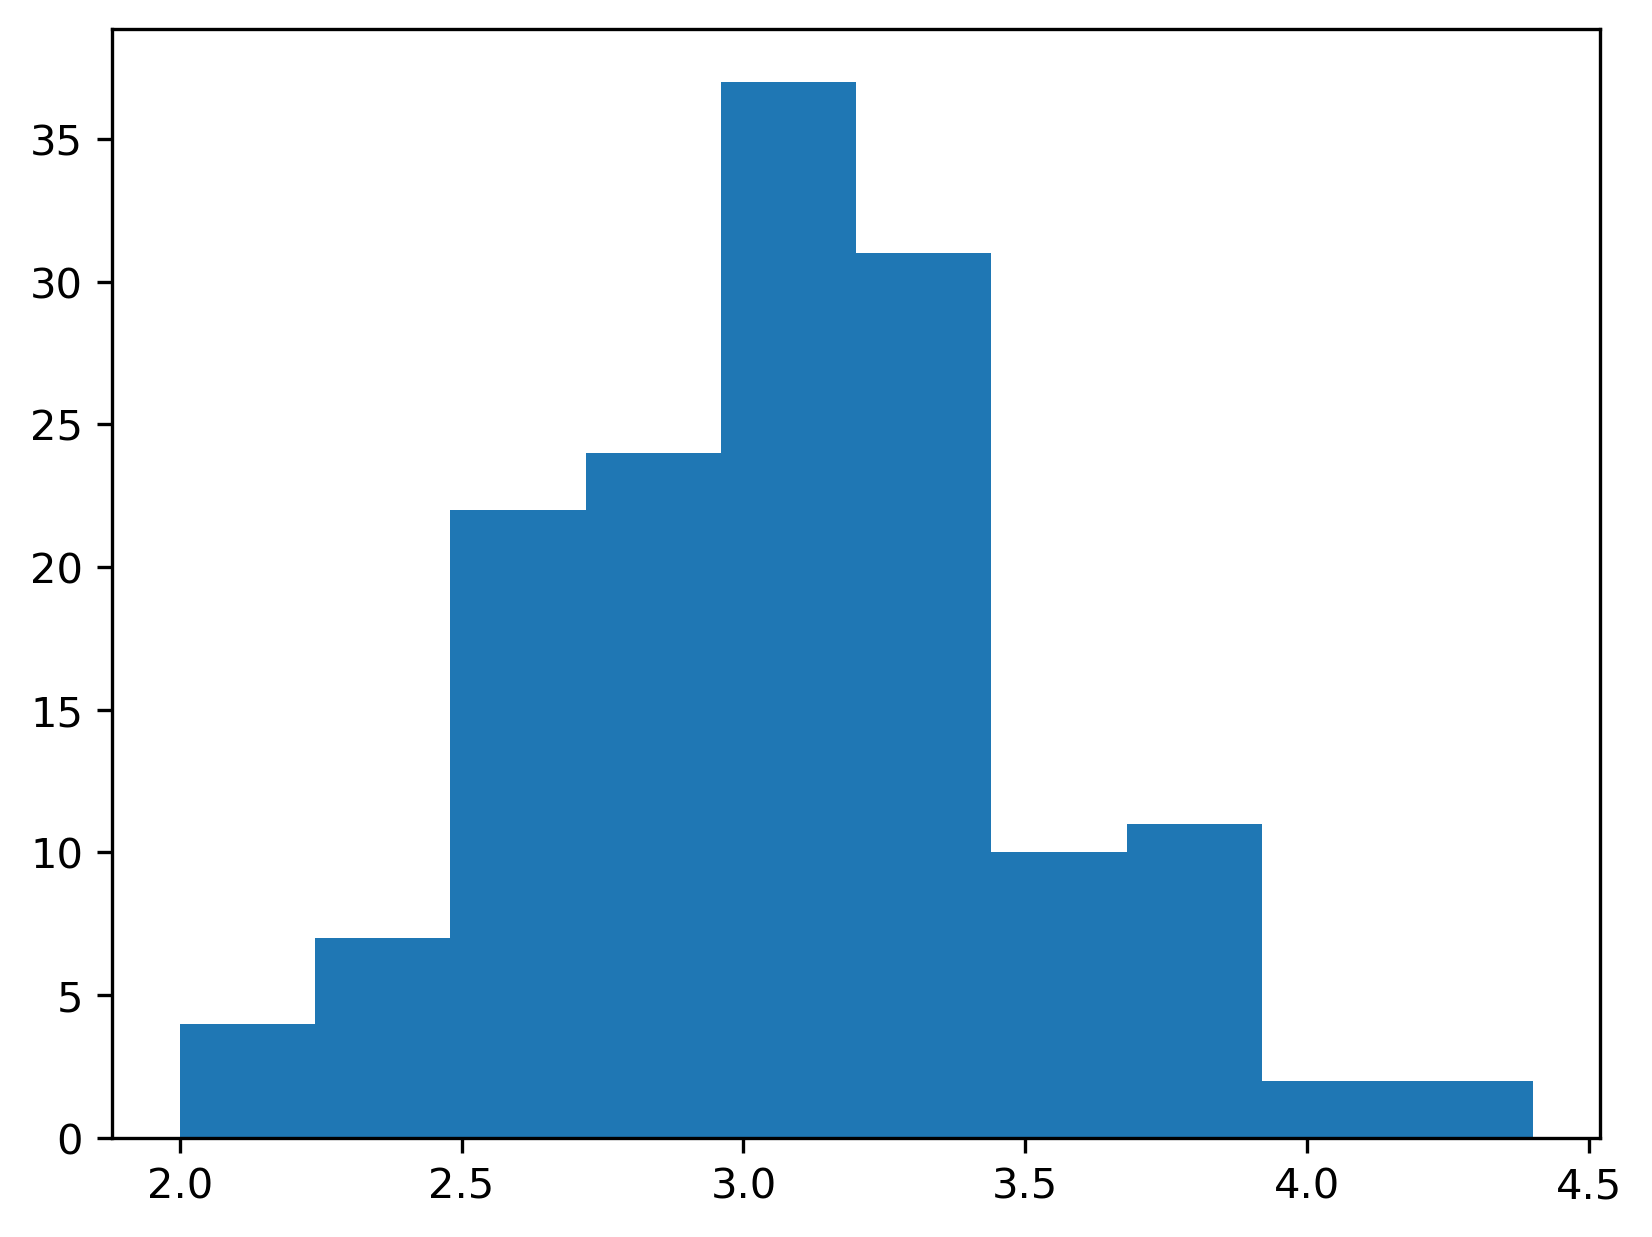
\includegraphics[]{sepal_width_histogram.png}
\end{figure}
\textbf{1b. Based on the histogram from \#1a, which would you expect to be higher, the mean or the median? Why?}
The histogram has 10 bins so you can split the distribution into 2 parts - the left 5 bins and the right 5 bins. If you compare these parts one bin at a time moving out from the center (5-6, 4-7, 3-8, 2-9, 1-10) then you'll notice that the left bin is always higher than its corresponding right bin. That means we have a distribution which is biased towards the left. If we consider a different left-biased distribution where 90\% of the values are at 0 and the remaining 10\% of values are at 1 then it's obvious that the median will be 0 and the mean will be greater than 0 in this new distribution. Thus in our original distribution which is also left-biased we would expect the same result - the mean is higher than the median.
\textbf{1c. Confirm your answer to \#1b by actually finding these values.}
\begin{verbatim}
print("Mean: ", iris['sepal width (cm)'].mean(), "\nMedian: ", iris['sepal width (cm)'].median())
>Mean:  3.057333333333334 
>Median:  3.0
\end{verbatim}
Our median is exactly 3 and our mean is greater than 3 as we suspected.

\textbf{1d. Only 27\% of the flowers have a Sepal.Width higher than \_\_\_\_\_\_\_\_ cm.}
\begin{verbatim}
print("top 27% of sepal widths (73rd percentile): ", iris['sepal width (cm)'].quantile(q=0.73))
>top 27% of sepal widths (73rd percentile):  3.3
\end{verbatim}
3.3 however doesn't exactly answer the question as asked since it specifies that *only* the top 27\% are in this group.
let's check around this value.
\begin{verbatim}
print(len(iris[iris['sepal width (cm)']>=3.3])/len(iris['sepal width (cm)']))
>0.2866666666666667
print(len(iris[iris['sepal width (cm)']> 3.3])/len(iris['sepal width (cm)']))
>0.24666666666666667
\end{verbatim}
If we include every value above 3.3 we only have 24.6\% of values but if we also include 3.3 itself then we now have 28.6\% of values. Therefore we can conclude that the question as asked is unanswerable - there is no way to define a meaningful line that includes only the top 27\% of this data set.

\textbf{1e. Make scatterplots of each pair of the numerical variables in iris (There should be 6 pairs/plots).}
\begin{verbatim}
figure, axis = pyplot.subplots(3, 2)
for i, combination in enumerate(combinations(['sepal length (cm)', 'sepal width (cm)', 
                                              'petal length (cm)', 'petal width (cm)'],2)):
    axis[i%3,i%2].scatter(iris[combination[0]],iris[combination[1]])
    axis[i%3,i%2].axes.set_xlabel(combination[0])
    axis[i%3,i%2].axes.set_ylabel(combination[1])
figure.tight_layout()
pyplot.savefig("multiplot.png", format = "png", dpi=300, bbox_inches="tight")
pyplot.clf()
\end{verbatim}
\begin{figure}
    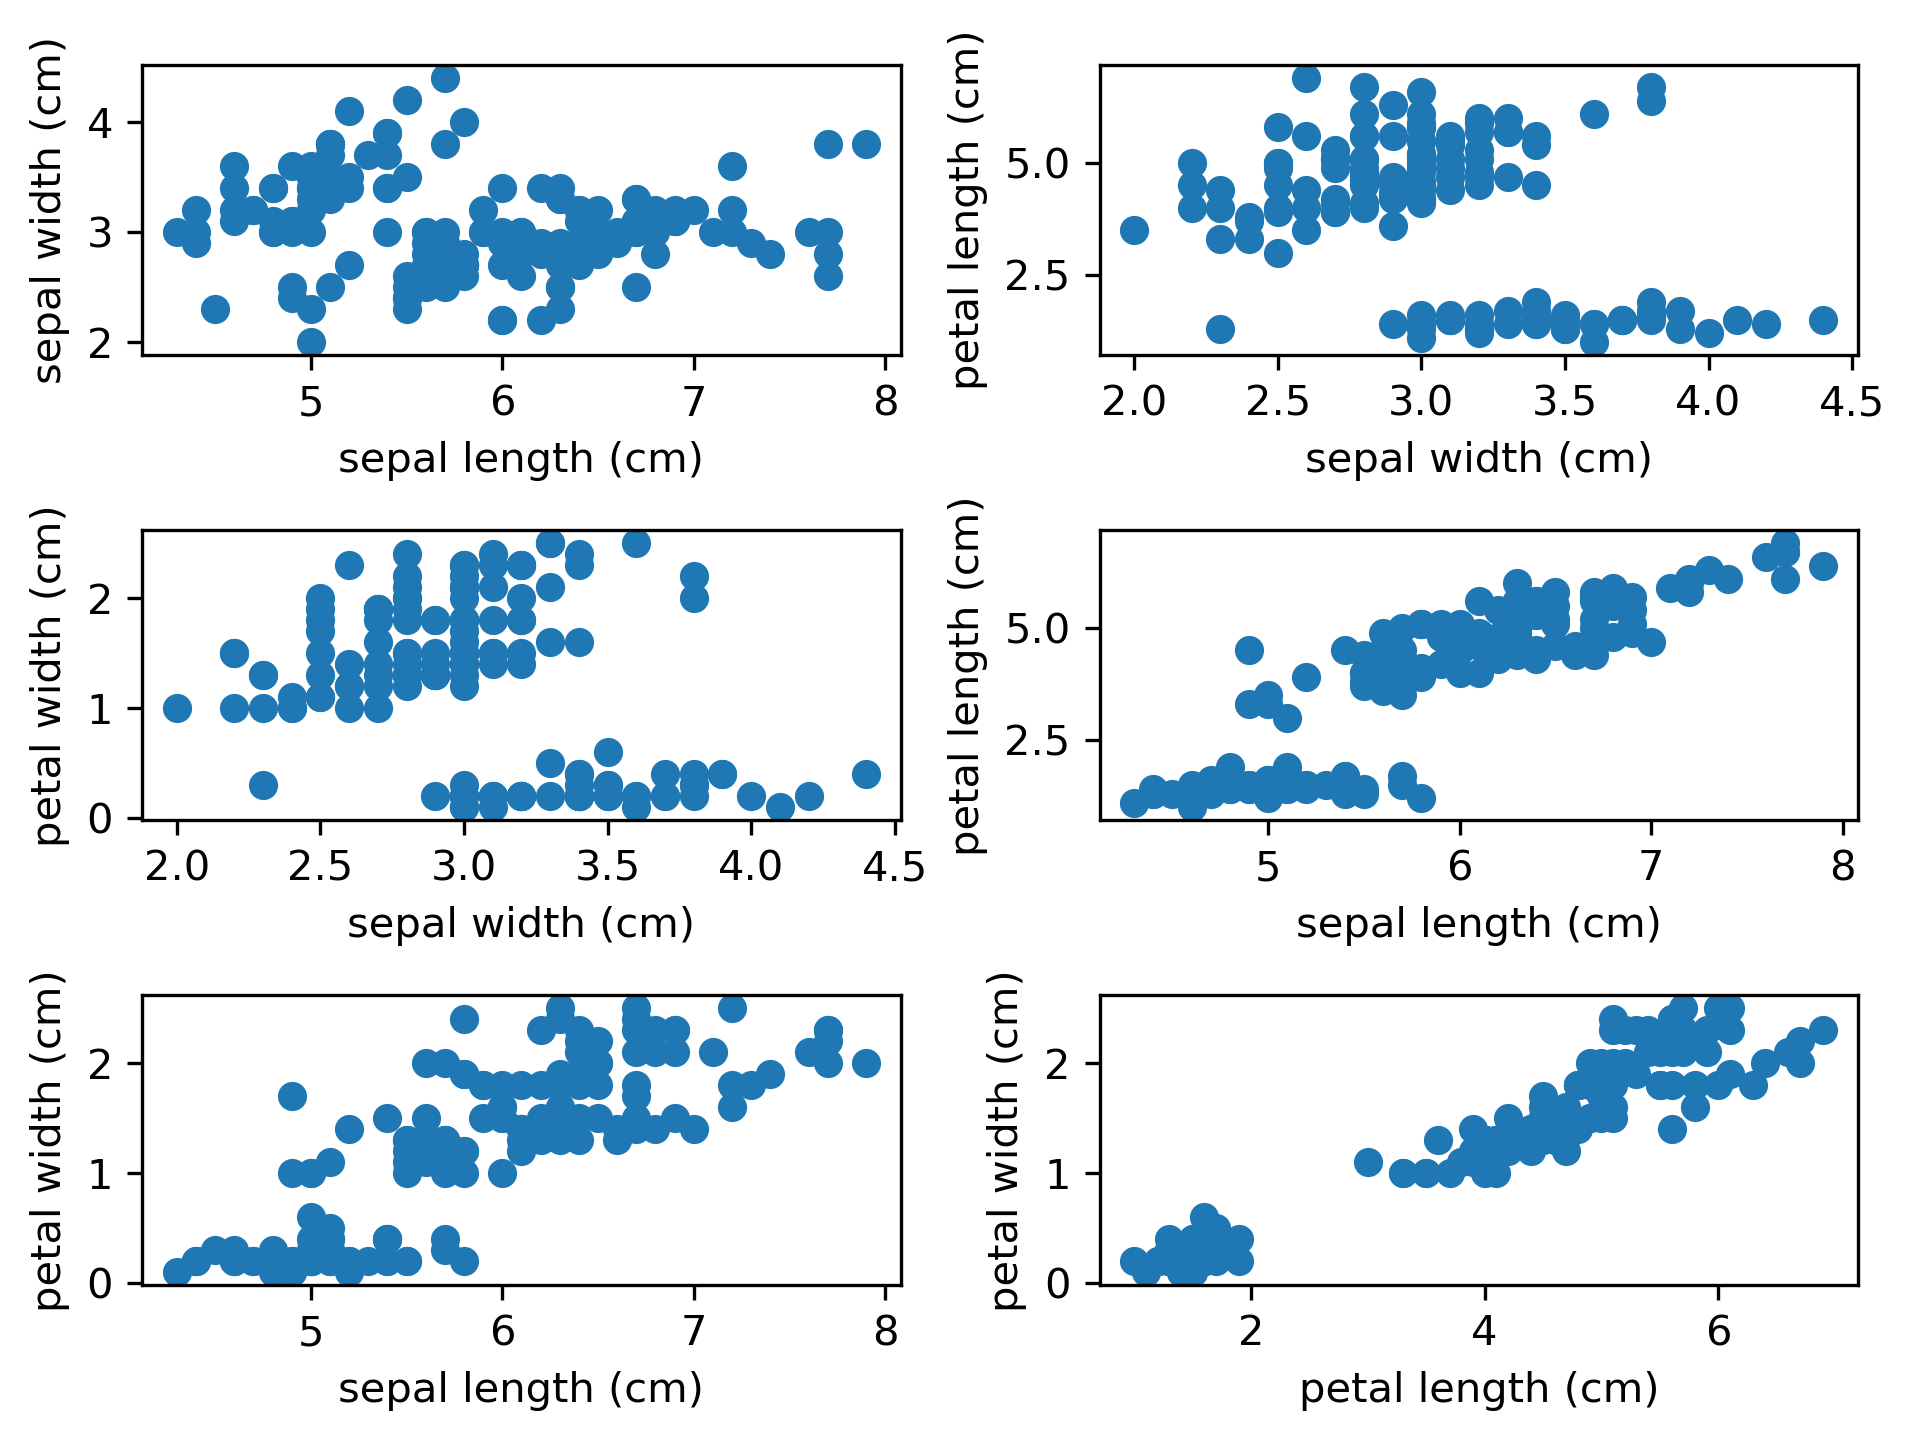
\includegraphics[]{multiplot.png}
\end{figure}
\textbf{1f. Based on \#1e, which two variables appear to have the strongest relationship? And which two appear to have the weakest relationship?}
Petal length and petal width (bottom right) appears to have the strongest correlation in this data set. There's a gap in the data but aside from that it's a pretty tight linear relationship with low noise.

The weakest relationship is harder since many of the plots appear to be multi modal. Sepal width vs petal length (top right) for example has 2 fairly distinct groupings but each group has a different relationship and the lower grouping has essentially 0 correlation. If all of the data needs to be considered though sepal length vs sepal (top left) width has the lowest correlation overall in that if you knew one you wouldn't gain much information about the other.
\textbf{2a. Make a histogram of the variable weight with breakpoints (bin edges) at every 0.3 units, starting at 3.3.}
\begin{verbatim}
bin_ticks = np.arange(3.3, max(PlantGrowth['weight'])+0.3, 0.3)
pyplot.hist(PlantGrowth['weight'], bins = bin_ticks)
pyplot.xticks(bin_ticks)
pyplot.savefig("weight_hist.png", format = "png", dpi=300, bbox_inches="tight")
\end{verbatim}
\begin{figure}
    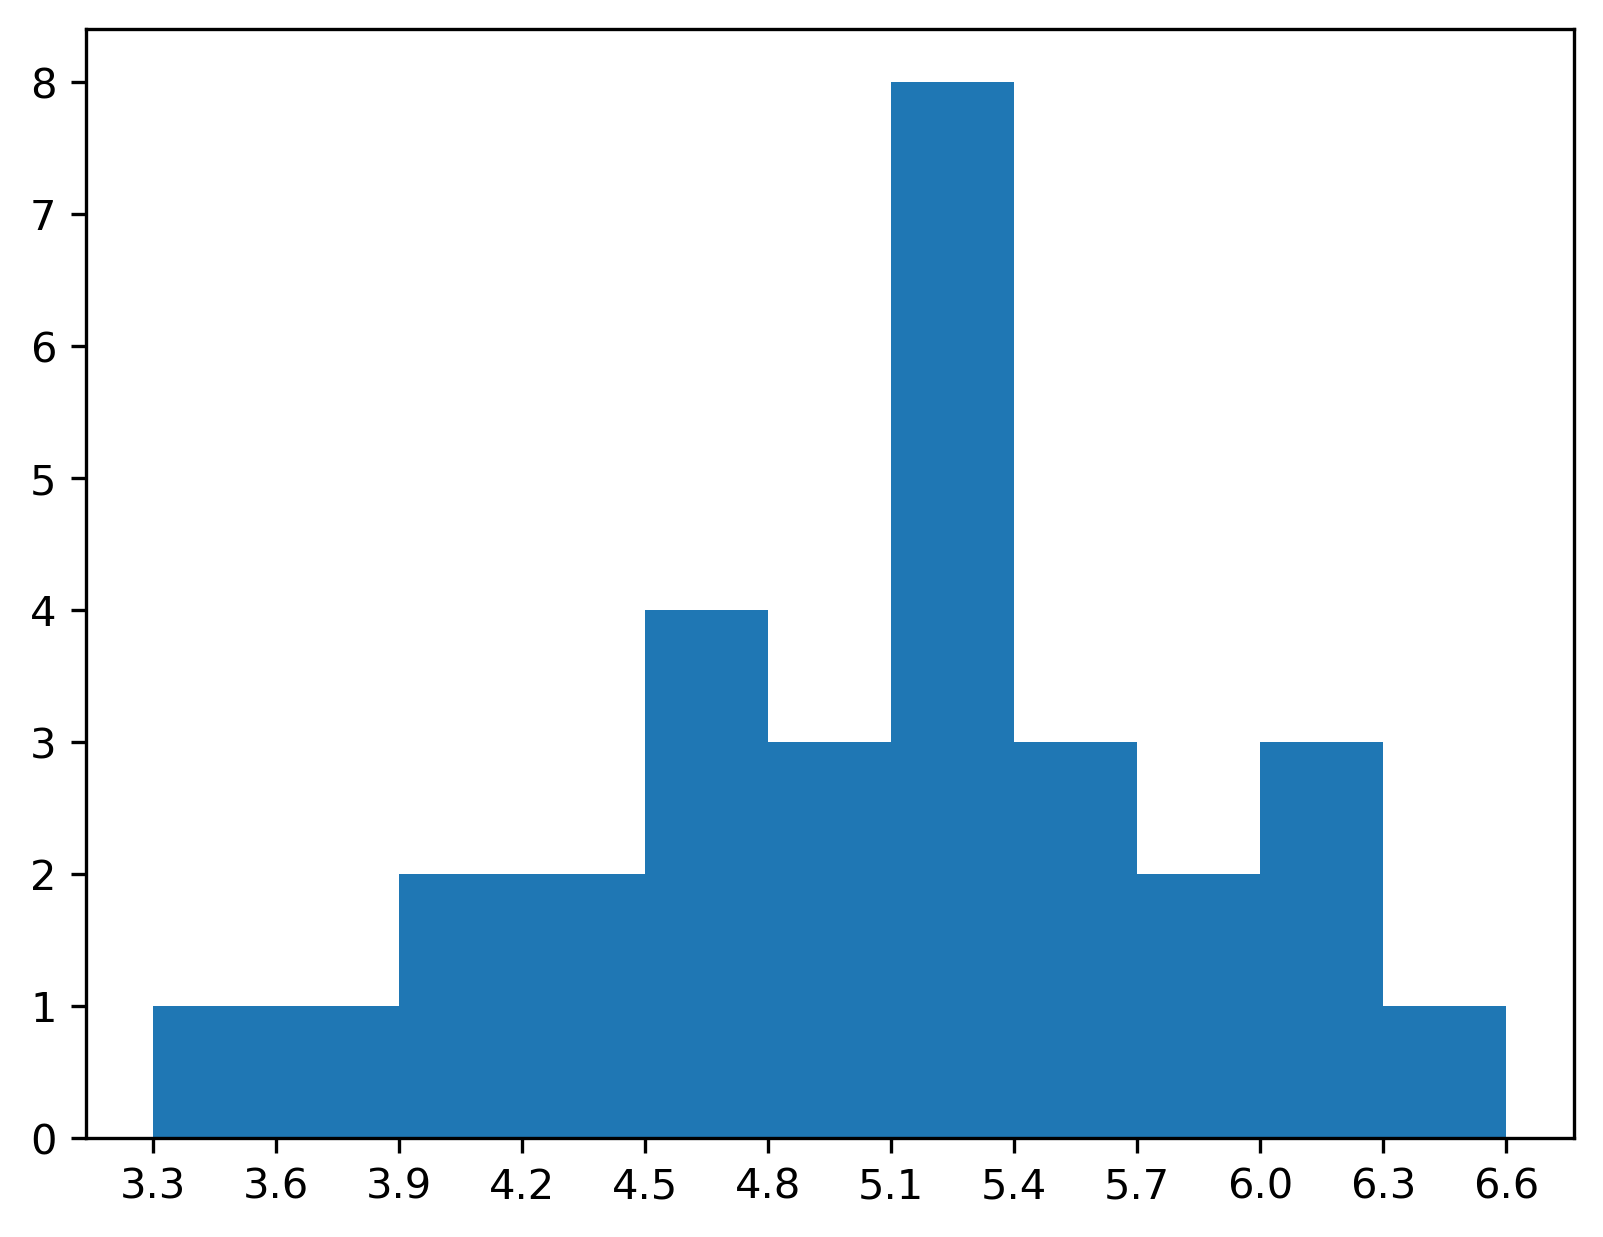
\includegraphics[]{weight_hist.png}
\end{figure}
\textbf{2b. Make boxplots of weight separated by group in a single graph.}
\begin{verbatim}
figure, axis = pyplot.subplots(1, 3)
for i,group in enumerate(PlantGrowth['group'].unique()):
    group_data = PlantGrowth[PlantGrowth['group'] == group]
    axis[i].boxplot(group_data['weight'])
    axis[i].axes.set_xlabel(group)
    axis[i].set_xticks([])
    axis[i].set_ylim(3.5,6.5)
figure.tight_layout()
pyplot.savefig("weight_box.png", format = "png", dpi=300, bbox_inches="tight")
\end{verbatim}
\begin{figure}
    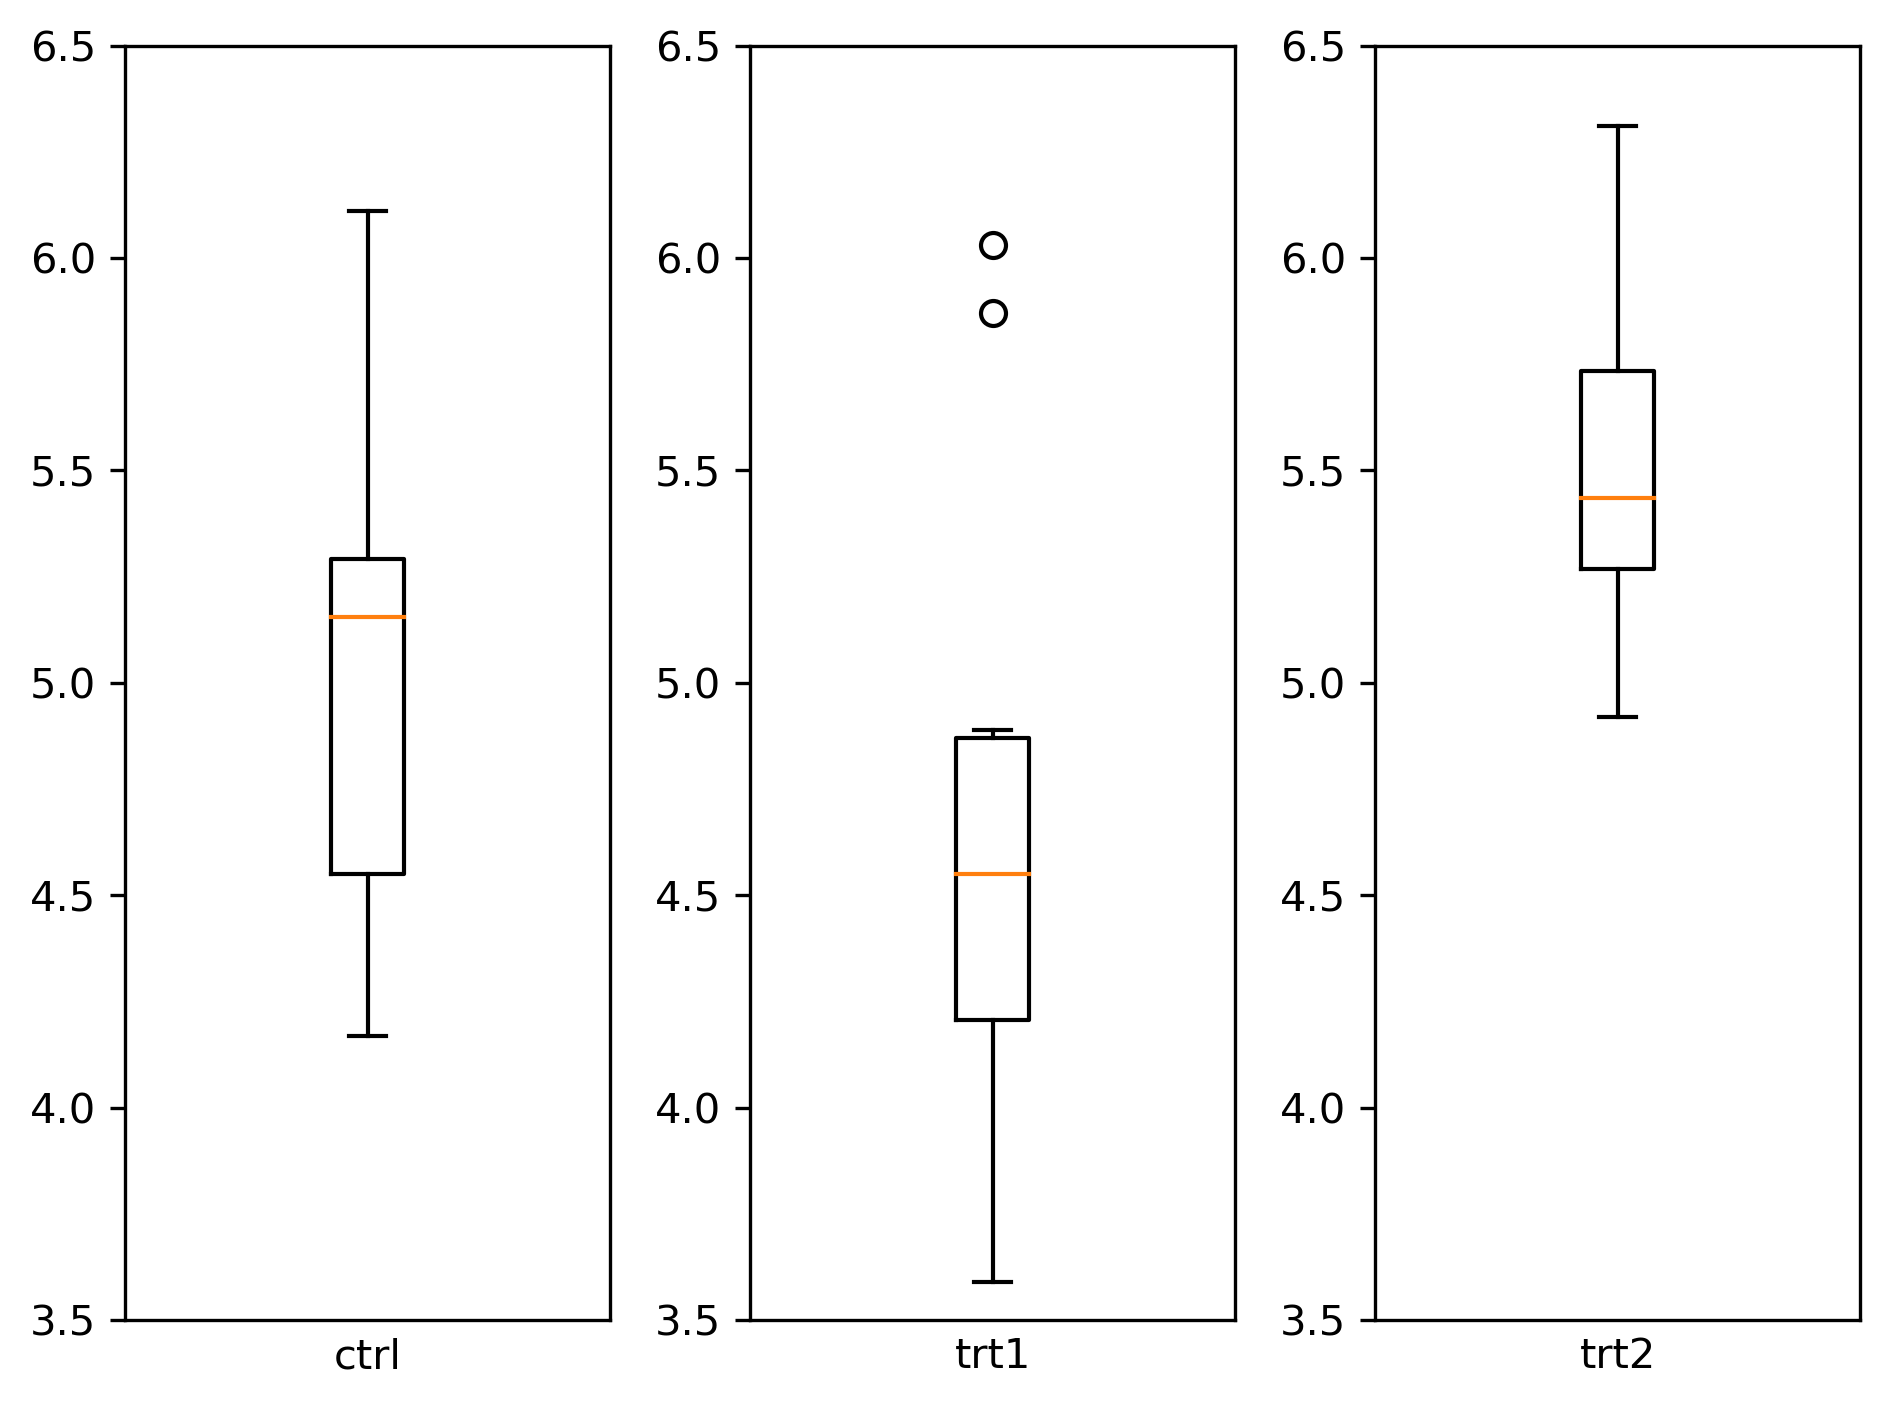
\includegraphics[]{weight_box.png}
\end{figure}
\textbf{2c. Based on the boxplots in \#2b, approximately what percentage of the "trt1" weights are below the minimum "trt2" weight?}
There are 10 data points in each group and the entire box plot for trt1 is below trt2. That means that only the 2 outliers are inside the trt2 range. Given that I'd expect exactly 80\% of of trt1 weights are below trt2 weights.
\textbf{2d. Find the exact percentage of the "trt1" weights that are below the minimum "trt2" weight.}
\begin{verbatim}
cutoff = min(PlantGrowth[PlantGrowth['group']=='trt2']['weight'])
below = len(PlantGrowth[(PlantGrowth['group']=='trt1') & (PlantGrowth['weight'] < cutoff)])
total = len(PlantGrowth[PlantGrowth['group']=='trt1'])
print(below/total*100,'%', sep="")
>80.0%
\end{verbatim}
\textbf{2e. Only including plants with a weight above 5.5, make a barplot of the variable group. Make the barplot colorful using some color palette}
\begin{verbatim}
heavy = PlantGrowth[PlantGrowth['weight']>5.5]
pyplot.bar(heavy['group'], heavy['weight'].mean())
print(heavy['weight'])
pyplot.savefig("heavy_bar.png", format = "png", dpi=300, bbox_inches="tight")
\end{verbatim}
\begin{figure}
    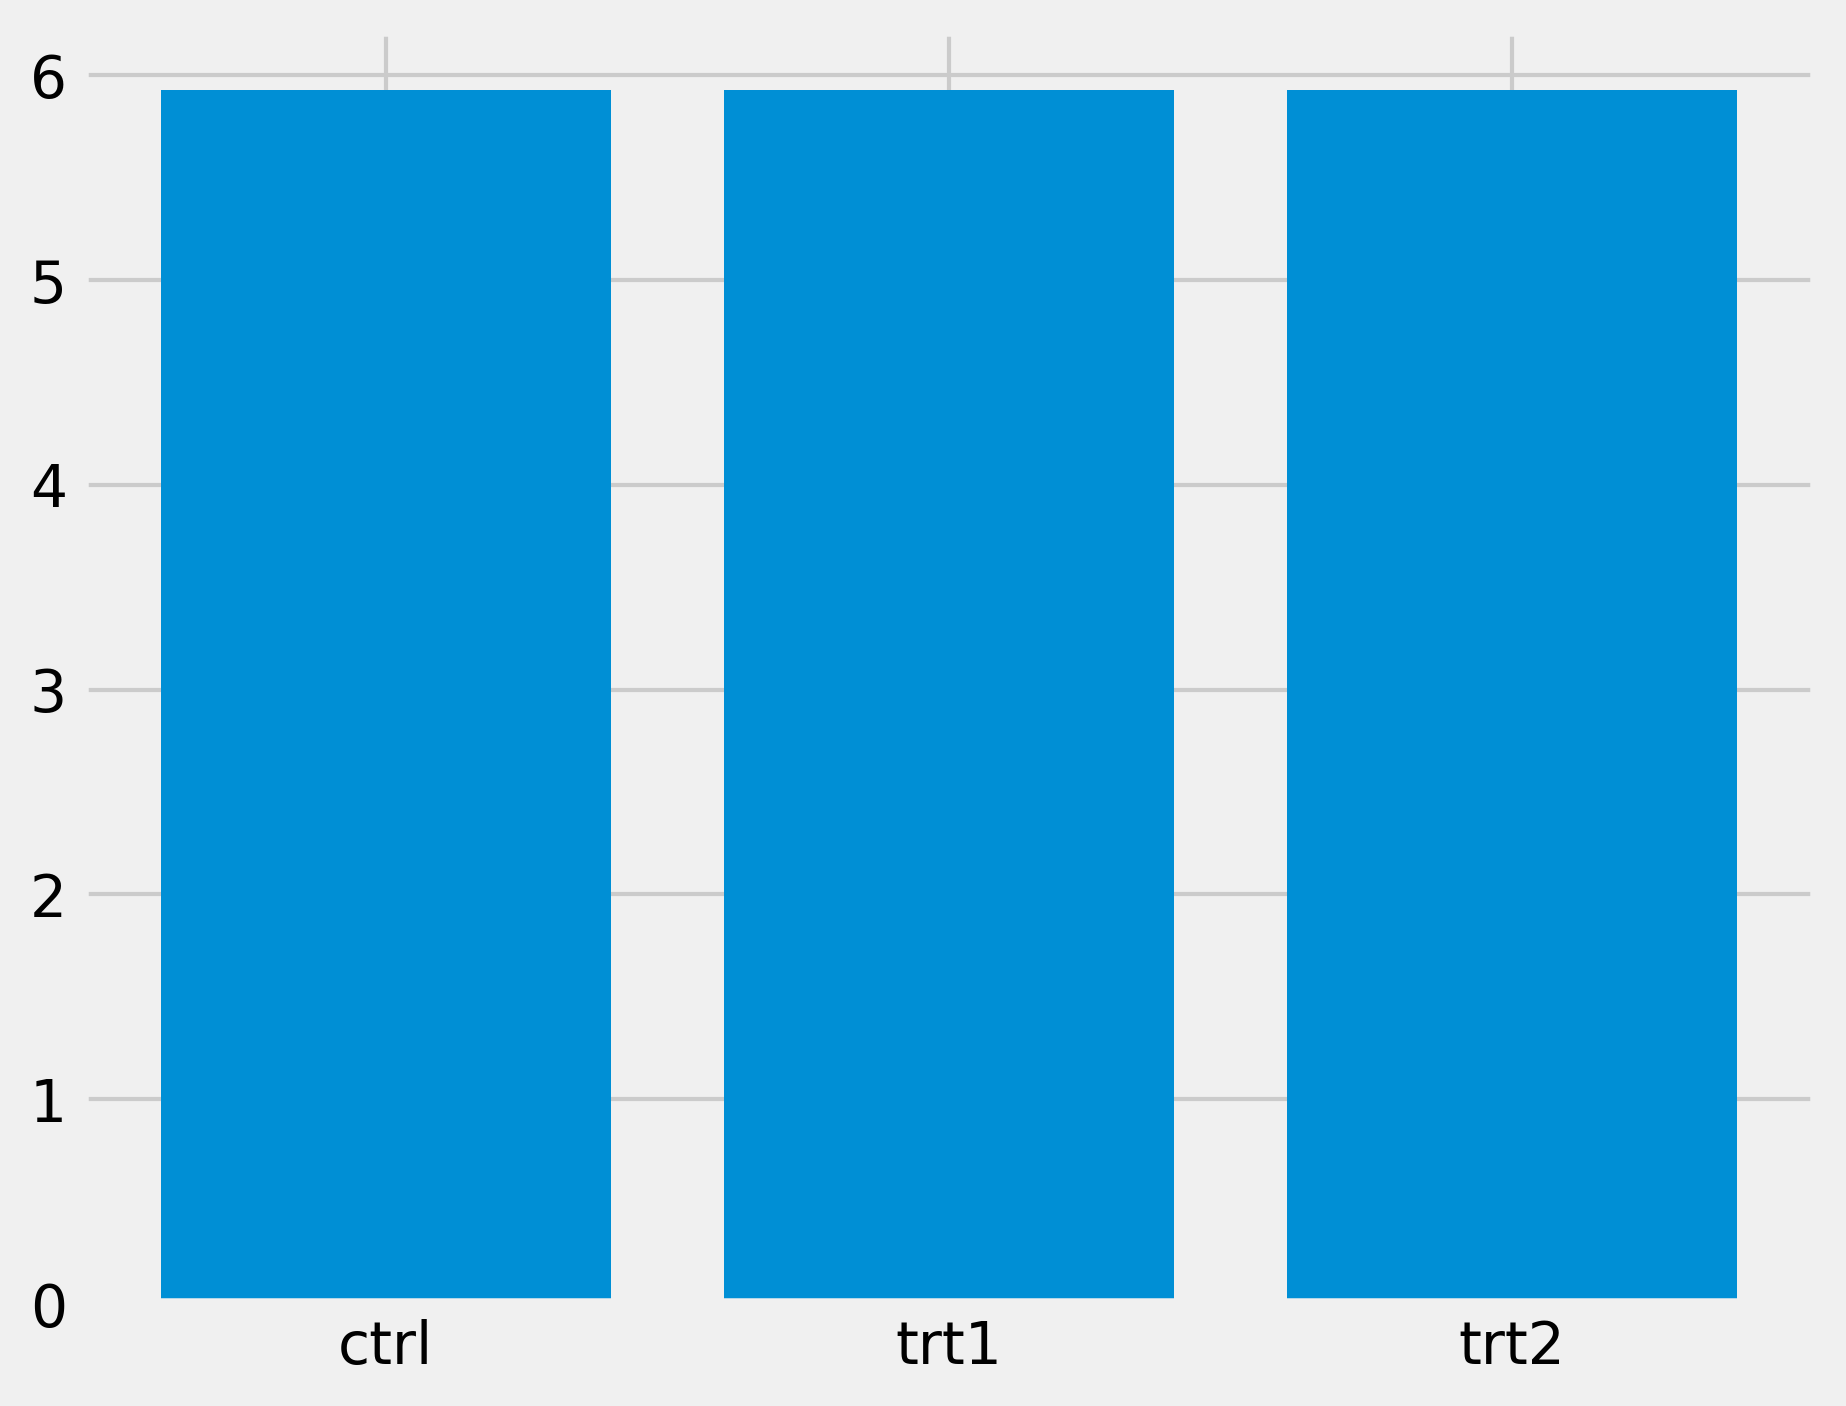
\includegraphics[]{heavy_bar.png}
\end{figure}
\end{document}